\documentclass[12pt,a4paper,titlepage]{scrartcl}

\usepackage{comment}
\usepackage[main=ngerman,english]{babel}
\usepackage[utf8]{inputenc}
\usepackage[T1]{fontenc}
\usepackage{lmodern}
\usepackage{geometry}
\geometry{left=2.5cm,right=2.5cm,top=2.5cm,bottom=3cm,head=29pt,foot=25pt}
\setlength{\footheight}{25pt}
\usepackage{microtype}
\usepackage{amsmath,amssymb,mathtools}
\numberwithin{equation}{section}
\numberwithin{table}{section}
\numberwithin{figure}{section}
\usepackage{siunitx}
\sisetup{locale=US, separate-uncertainty=true, per-mode=fraction}
\usepackage{booktabs}
\usepackage{multirow}
\usepackage{graphicx}
\usepackage{float}
\usepackage{caption}
\usepackage{subcaption}
\usepackage[automark]{scrlayer-scrpage}
\usepackage[most]{tcolorbox}
\usepackage{hyperref}
\usepackage{pdfpages}
\usepackage{csvsimple-l3}
\usepackage{longtable}
\usepackage{graphicx}

%\input{../../jupyterpackages.tex}

% jupyter nbconvert --to latex 'Path'
% enferne usepackages und begin{document} und end{document}
% \input in main.tex mit \input{Path}


\newcommand{\pdfabbildung}[2]{%
    \refstepcounter{figure}%
    \addcontentsline{lof}{figure}{\protect\numberline{\thefigure}#1}%
    \label{#2}%
}

\newcommand{\pdftabelle}[2]{%
    \refstepcounter{table}%
    \addcontentsline{lot}{table}{\protect\numberline{\thetable}#1}%
    \label{#2}%
}


\hypersetup{colorlinks=true, linkcolor=blue!60!black, urlcolor=blue!60!black, citecolor=blue!60!black}

\clearpairofpagestyles

\chead{%
    \versuch\hfill\autor\\
    \rule{\textwidth}{0.2pt}%
}
\cfoot{%
    \rule{\textwidth}{0.2pt}\\[-0.5ex]
    \pagemark\ 
}
\addtokomafont{pagefoot}{\small}
\setlength{\parindent}{0pt}

\newtcolorbox{resultbox}[1][]{ 
    enhanced,
    colback=black!4!white,
    colframe=black!65!black,
    boxrule=0.8pt,
    arc=0.0mm,
    title=#1,
    fonttitle=\bfseries,
    %drop shadow
}


\newcommand{\versuch}{Versuch 41}
\newcommand{\titel}{Temperaturmessung}
\newcommand{\praktikum}{Physikalisches Anfängerpraktikum 1}
\newcommand{\autor}{Jonathan Gießen}
\newcommand{\gruppe}{Gruppe 8}
\newcommand{\datum}{31. September 2026}
\newcommand{\betreuer}{Furkan Cetin}

\begin{document}

\pagestyle{scrheadings}

\begin{titlepage}



    \centering
    \vspace*{4cm}
    {\large Universität Heidelberg\par}
    {\small Fakultät für Physik und Astronomie\par}
    {\Large \praktikum\par}
    \vspace{0.8cm}
    {\LARGE \bfseries \versuch\ -- \titel\par}
    \vspace{1.5cm}

    \begin{tabular}{ll}
        \textbf{Autor:} & \autor\\
        \textbf{Gruppe:} & \gruppe\\
        \textbf{Betreuer:} & \betreuer\\
        \textbf{Versuchsdatum:} & \datum\\
    \end{tabular}

    \vfill
    \hrulefill\
\end{titlepage}

\tableofcontents

\bigskip
\begin{tcolorbox}[colback=gray!5,colframe=gray!60,boxrule=0.8pt,arc=0.01mm,title=KI-Hinweis]
    Für die sprachliche Formulierung dieses Protokolls wurde in der Einleitung \ref{sec:Einleitung} KI-gestützte Textgenerierung verwendet. 
\end{tcolorbox}

\clearpage


\section{Einleitung}\label{sec:Einleitung}
Ziel dieses Versuchs ist es, verschiedene physikalische Prinzipien der Temperaturmessung in unterschiedlichen Messbereichen praktisch anzuwenden. Dazu werden vergleichende Messungen mit einem Gasthermometer und einem Platin-Widerstandsthermometer im Bereich zwischen den Siedepunkten von flüssigem Stickstoff und Wasser durchgeführt. Ergänzend erfolgen Messungen mit einem Infrarot-Thermometer im Temperaturbereich von 0 °C bis 100 °C. Zudem wird als typische Anwendung eines Thermoelements die Temperaturverteilung einer Bunsenbrennerflamme mithilfe eines PtRh-Elementes bestimmt.

\section{Grundlagen und Theorie}\label{sec:Grundlagen}
Thermometer sind Geräte, die zur Messung der Temperatur verwendet werden. Sie basieren auf verschiedenen physikalischen Prinzipien, die es ermöglichen, die Temperatur eines Systems zu bestimmen. 

\subsection{Gasthermometer}\
Das Gasthermometer ist ein Gerät, das die Temperatur durch die Messung des Drucks eines Gases bei konstantem Volumen bestimmt. Es basiert auf dem idealen Gasgesetz, das den Zusammenhang zwischen Druck, Volumen und Temperatur beschreibt. Bei konstantem Volumen ist der Druck direkt proportional zur Temperatur. Daher kann die Temperatur durch die Messung des Drucks des Gases ermittelt werden.

\begin{align}
    &pV = nRT\\
    \Rightarrow\  &p \propto T \quad \text{bei konstantem Volumen}
\end{align}

\begin{figure}[H]
    \centering
    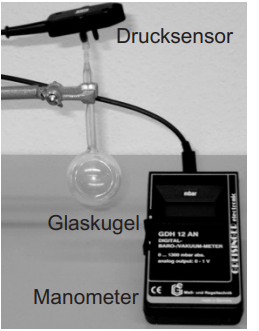
\includegraphics[width=0.4\textwidth]{img/Gasthermometer.png}
    \caption{Schematische Darstellung eines Gasthermometers.\cite{PAPskript}}
    \label{fig:gasthermometer}

\end{figure}


\subsection{Das Thermoelement}
Das Thermoelement beruht einen auf den Seebeck-Effekt, der besagt, dass in einem geschlossenen Stromkreis aus zwei unterschiedlichen Metallen eine Spannung entsteht, wenn die beiden Verbindungsstellen unterschiedliche Temperaturen haben. Diese Spannung ist proportional zur Temperaturdifferenz zwischen den beiden Verbindungsstellen. Durch die Messung der erzeugten Spannung kann die Temperaturdifferenz bestimmt werden.


\begin{figure}[H]
    \centering
    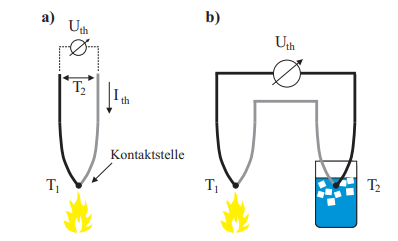
\includegraphics[width=0.4\textwidth]{img/Thermoelement.png}
    \caption{Schematische Darstellung eines Thermoelements.\cite{PAPskript}}
    \label{fig:thermoelement}
\end{figure}

\begin{equation}
    U_th = K  (T_1 - T_2)
\end{equation}
K ist dabei die Seebeck-Konstante, die von den verwendeten Metallen abhängt.
Problematisch ist, dass bei diesem Thermometer nur relative Temperaturdifferenzen gemessen werden können. Um absolute Temperaturen zu bestimmen, muss eine bekannte Referenztemperatur verwendet werden, was nicht immer leicht umzusetzten ist.

\subsection{Platin-Widerstandsthermometer}
Das Platin-Widerstandsthermometer basiert auf der Tatsache, dass der elektrische Widerstand von Platin mit der Temperatur variiert. Der Widerstand steigt mit zunehmender Temperatur an. Durch die Messung des Widerstands kann die Temperatur bestimmt werden.
Die Temperaturabhägigkeit des Widerstands von Platin kann durch die folgende Gleichung beschrieben werden:

\begin{align}
    R(T) = R_0  (1 + AT + BT^2)\label{eq:Widerstandpt100}
\end{align}

$R_0$ ist der Nennwiderstand bei 0 °C, A und B sind Konstanten, die die Temperaturabhängigkeit des Widerstands beschreiben. Die Werte für A und B können aus Literaturwerten entnommen werden.

Umgeformt nach T mit der Quadratischen Lösungsformel ergibt sich:
\begin{equation}
    T = \frac{-R_0  A + \sqrt{(R_0  A)^2 - 4  R_0  B  (R_0 - R)}}{2  R_0  B}
\end{equation}

Unser Platin-Widerstandsthermometer hat einen Nennwiderstand von $R_0 = 100\,\Omega$ bei 0 °C. Die Konstanten A und B sind in der Literatur angegeben und betragen $A = \qty{3.9083e-3}{\degreeCelsius}^{-1}$ und $B = \qty{-5.775e-7}{\degreeCelsius}^{-2}$. Die Genauigkeitsklasse des Thermometers beträgt Klasse B, was einer Genauigkeit von $\Delta T = 0.30\,\si{\degreeCelsius} + 0.005 \cdot \lvert T \rvert$ entspricht.

Mithilfe einer Vierleiter-Schaltung kann der Widerstand des Platin Widerstandsthermometers sehr genau gemessen werden. Dabei wird der Strom durch das Thermometer mit zwei Leitern geführt, während die Spannung über das Thermometer mit zwei weiteren Leitern gemessen wird. Dies minimiert den Einfluss des Leitungswiderstands auf die Messung.


\subsection{Pyrometer}
Das Pyrometer ist ein berührungsloses Thermometer, das die Temperatur eines Objekts durch die Messung der von ihm abgestrahlten Infrarotstrahlung bestimmt. Es basiert auf dem Planckschen Strahlungsgesetz, das beschreibt, wie die Intensität der Strahlung eines schwarzen Körpers von seiner Temperatur abhängt. Durch die Messung der Strahlungsintensität kann die Temperatur des Objekts bestimmt werden.

Mithilfe des Planckschen Strahlungsgesetzes wird die Intensitätsverteilung der Strahlung eines schwarzen Körpers in Abhängigkeit von der Wellenlänge und der Temperatur beschrieben. Die spektrale Strahldichte $M_\lambda(\lambda, T)$ eines schwarzen Körpers bei einer bestimmten Temperatur $T$ und Wellenlänge $\lambda$ wird durch die folgende Gleichung gegeben:

\begin{equation}
    M_\lambda(\lambda, T) \text{d}A\text{d}\lambda = \frac{2hc^2}{\lambda^5} \frac{1}{e^{\frac{hc}{\lambda k_B T}} - 1} \text{d}A\text{d}\lambda
\end{equation}

Durch Integration über die gesamte strahlende Fläche und über alle Wellenlängen kann die gesamte abgestrahlte Leistung $P$ eines schwarzen Körpers bei einer bestimmten Temperatur $T$ berechnet werden \cite{PAPskript}:
\begin{equation}
    P(T) = \epsilon(T)\sigma A T^4
\end{equation}

wobei $\epsilon(T)$ der Emissionsgrad des Materials ist, $\sigma$ die Stefan-Boltzmann-Konstante und $A$ die Fläche des strahlenden Körpers. Das Pyrometer misst die abgestrahlte Leistung und kann daraus die Temperatur des Objekts bestimmen.

Bei Zimmertemperatur $\approx 300$\,K liegt das Strahlungsmaximum im Infrarotbereich bei einer Wellenlänge von etwa 10 µm. In diesem Bereich arbeiten kommerzielle IR-Pyrometer. Die im Praktikum eingesetzten Pyrometer integrieren die von einem Körper ausgehende Strahlung im Bereich von 8 µm bis 14 µm. \cite{PAPskript}

\begin{figure}[H]
    \centering
    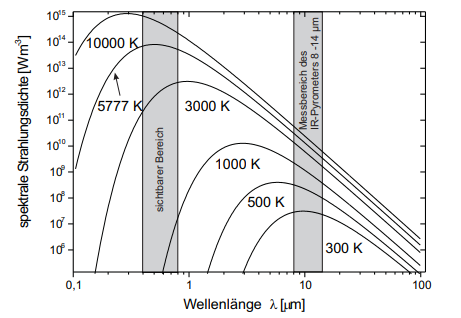
\includegraphics[width=0.4\textwidth]{img/Spektral intensity.png}
    \caption{Spektrale Intensitätsverteilung eines schwarzen Körpers bei unterschiedlichen Temperaturen.\cite{PAPskript}}
    \label{fig:strahlvertielung}
\end{figure}


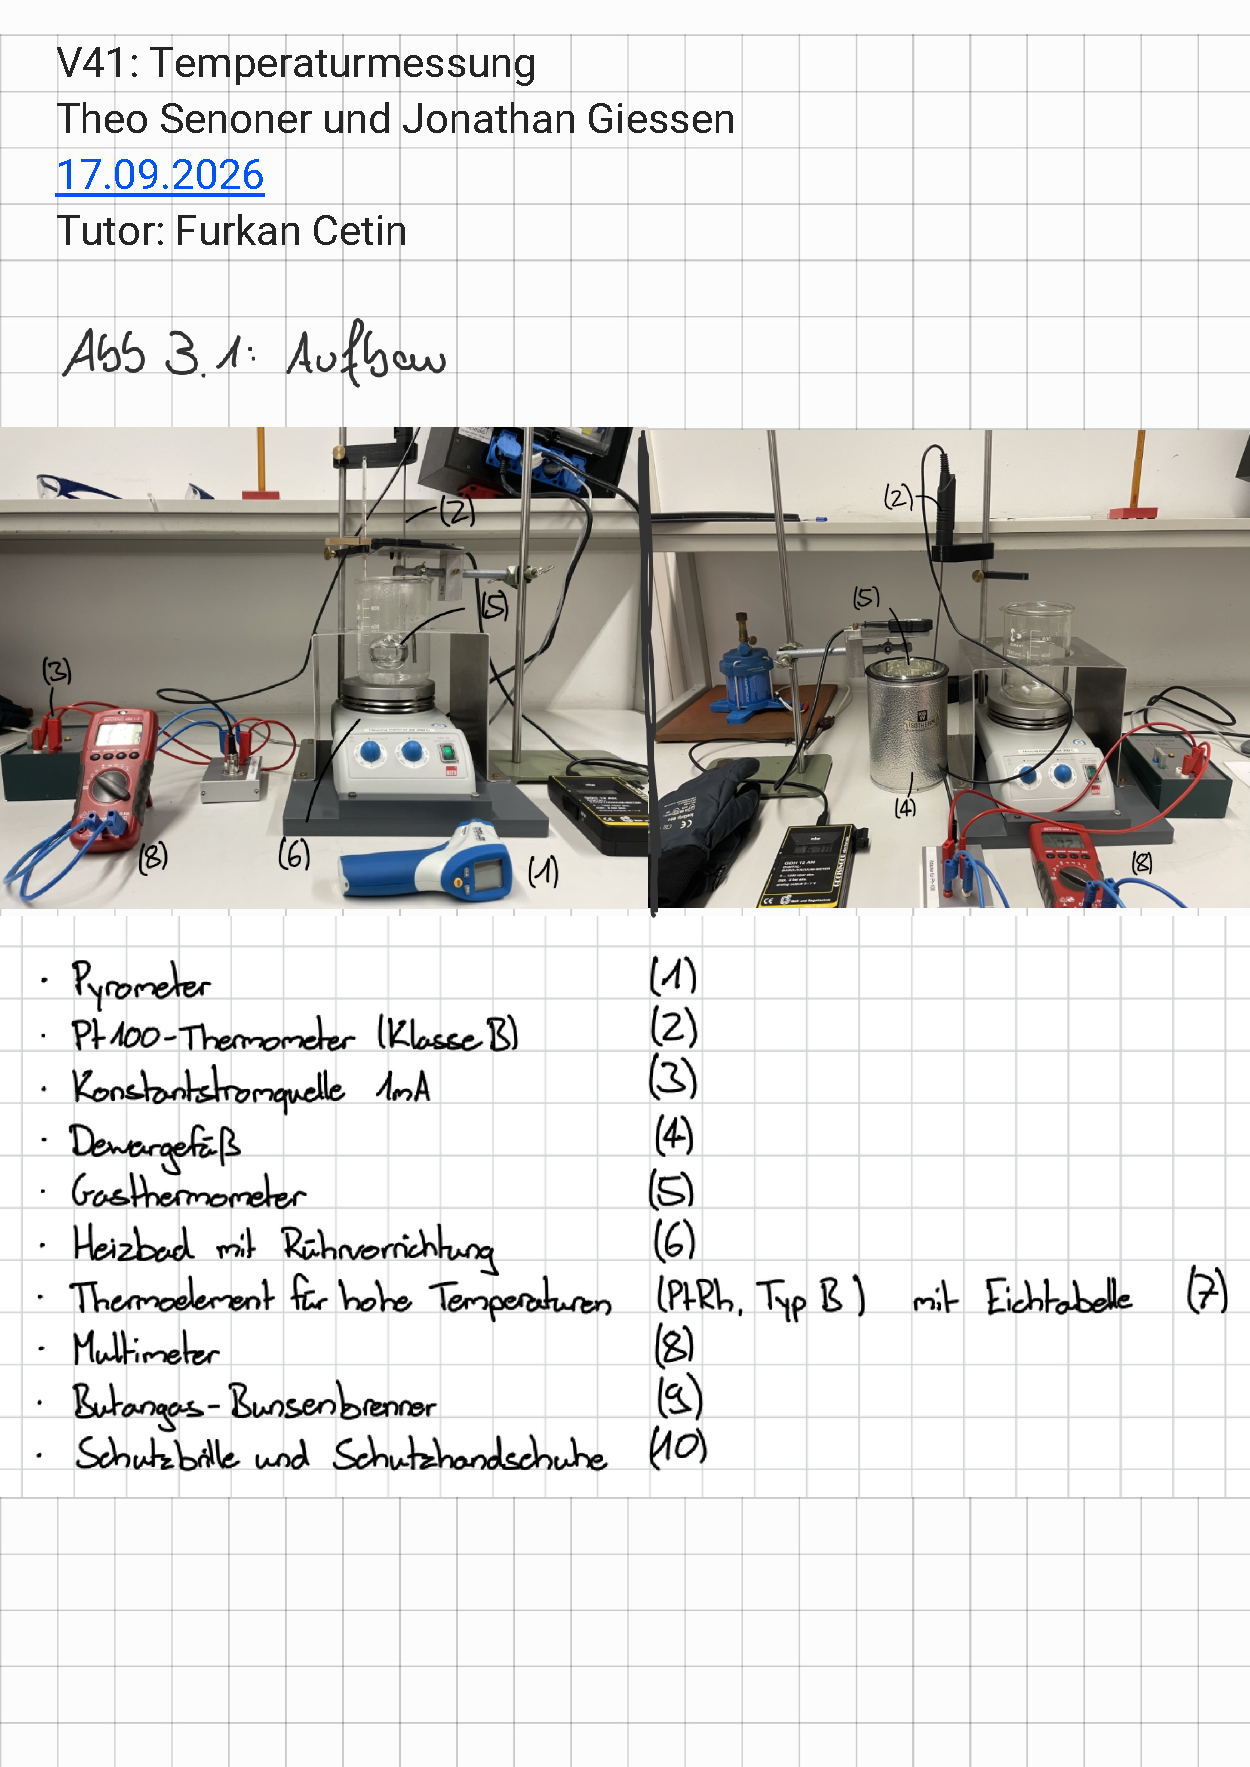
\includepdf[
    pages=1-4,
    width=\textwidth,
    height=0.95\textheight,
    keepaspectratio,
    pagecommand={\thispagestyle{scrheadings}},
    pagecommand*={\thispagestyle{scrheadings}\section{Messprotokoll}\subsection{Versuchsaufbau und Aufgaben}}
]{../Messprotokoll 41.pdf}

\begin{figure}
    \centering
    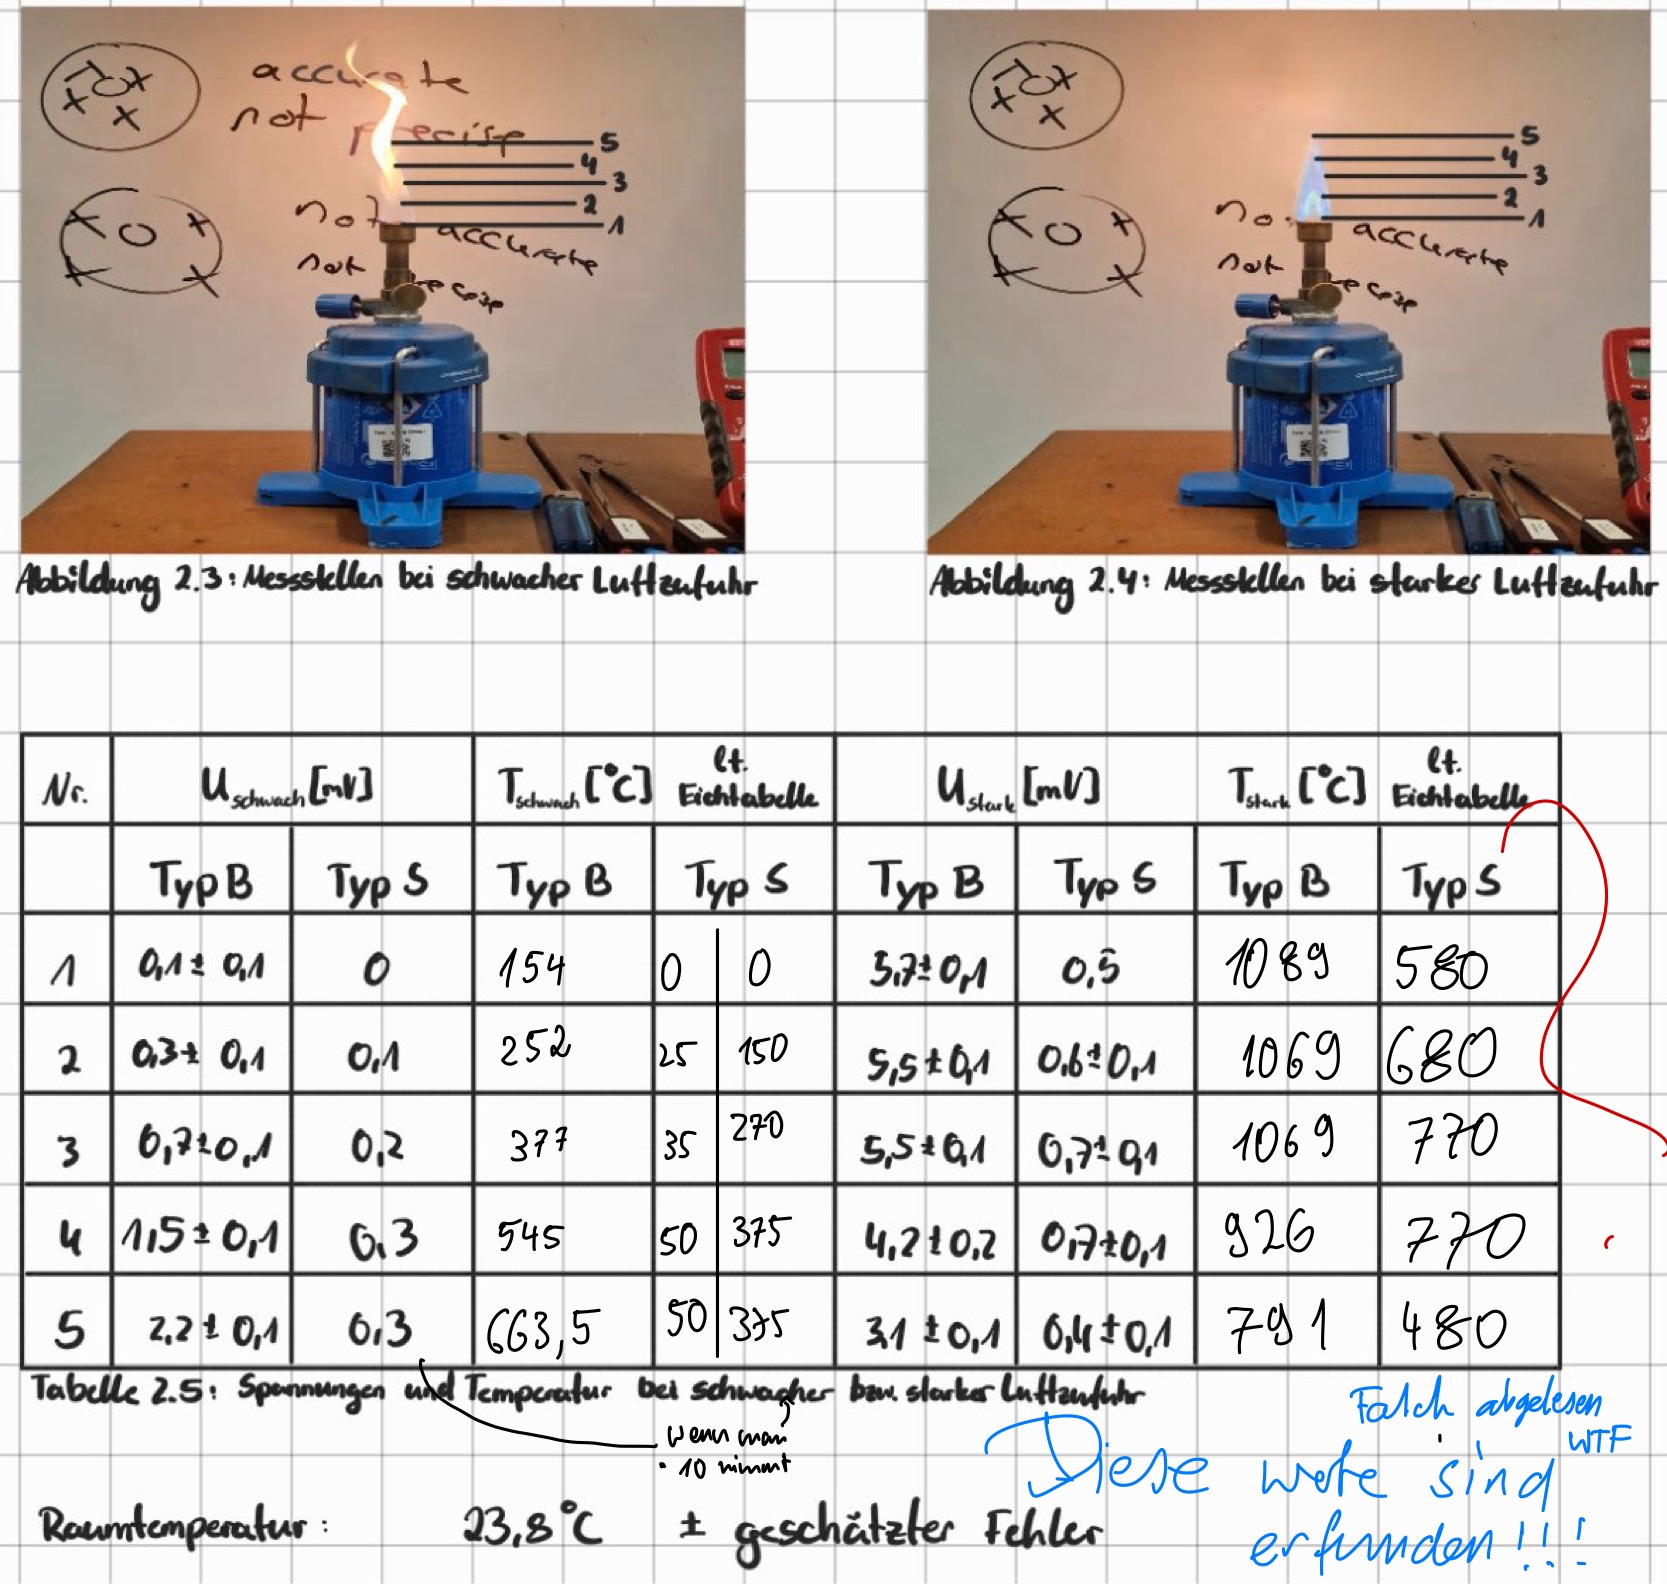
\includegraphics[width=0.8\textwidth]{img/V41_No4.jpg}
    \caption{Aufgabe 4: Messung der Temperaturverteilung in einer Bunsenbrennerflamme mit einem PtRh-Thermoelement.}
\end{figure}      


\subsection{Durchführung}
\paragraph{Aufgabe 1:} Eichung der Thermometer bei 0°C
Das Pt100-Thermometer wird als Vierleiterschaltung angeschlossen. Anschließend werden das Pt100-Thermometer, das Gasthermometer und das Pyrometer in einer Wasser-Eis-Mischung bei 0 °C kalibriert, indem die Spannung, der Druck und die angezeigte Temperatur notiert werden.

\paragraph{Aufgabe 2:} Temperaturmessung bis $T = 100$\,°C
Das Wasserbad wird auf einer Heizplatte bis zum Siedepunkt erhitzt. Im 10-Grad-Schritten werden jeweils die Spannung am Pt100, der Druck des Gasthermometers und die Pyrometeranzeige registriert.

\paragraph{Aufgabe 3:} Temperatur von Trockeneis und flüssigem Stickstoff am Siedepunkt
Der Glasballon und das Pt100 werden zunächst in einem Dewargefäß in einer Trockeneis-Alkohol-Mischung und in einer zweiten Messung in flüssigem Stickstoff abgekühlt. Nach der Stabilisierung werden jeweils die Pt100-Spannung und der Druck des Gasthermometers gemessen (das Pyrometer ist hier nicht einsetzbar).

\paragraph{Aufgabe 4:} Messung von sehr hohen Temperaturen mit dem PtRh-Thermoelement
Diese Messung wird vom Tutor vorgeführt. Mit einem PtRh-Thermoelement wird die Temperaturverteilung in einer Bunsenbrennerflamme bei starker und schwacher Luftzufuhr ausgemessen.


\section{Auswertung}
\subsection{Eintragen der Druckwerte gegen die Temperatur}
Zuerst wird das Gasthermometer geeicht. Dazu werden die Druckwerte bei 0 °C und 100 °C aus dem Messprotokoll gegen die Temperatur aufgetragen. Mithilfe von zwei Eichpunkten wird eine Gerade bestimmt.

Der Ablesefehler des Drucks $p_\text{abl} = 0.5\, mbar$ und der Gerätefehler von $\Delta p_\text{ger} = 2\, mbar$ addieren sich zu einem Gesamtfehler von:
\begin{equation}
    \Delta p = \sqrt{p_\text{abl}^2 + \Delta p_\text{ger}^2} = \sqrt{(0.5\,\text{mbar})^2 + (2\,\text{mbar})^2} \approx 2.1\,\text{mbar}
    \label{eq:druckfehler}
\end{equation}

Aus dem Messprotokoll wird der Druck $p_0 = 906\, \si{\milli\bar}$ bei 0 °C abgelesen und  $p_{sieden} = \qty{1241.0(2.1)}{\milli\bar}$ beim Sieden des Wassers abgelesen:

Da die Siedetemperatur abhängig vom Umgebungsluftdruck $p_\text{LD} = \qty{1006.0(2.0)}{\milli\bar}$ ist, muss der Druck auf den Normaldruck von $p_\text{norm} = 1013.25\,\si{\milli\bar}$ korrigiert werden:
\begin{equation}
    p_\text{NB} = p_\text{sieden} \frac{1013.25\,\si{\milli\bar}}{p_\text{LD}} \approx \qty{1250(4)}{\milli\bar}\footnotemark
\end{equation}
\footnotetext{Das ist eigentlich eine sehr fehlerbehaftete Näherung oder?}

mit der Fehlerfortpflanzung:
\begin{equation}
    \Delta p_\text{NB} = p_\text{sieden} \frac{1013.25\,\si{\milli\bar}}{p_\text{LD}} \sqrt{\left(\frac{\Delta p_\text{sieden}}{p_\text{sieden}}\right)^2 + \left(\frac{\Delta p_\text{LD}}{p_\text{LD}}\right)^2} = 3.26\,\si{\milli\bar} \approx \qty{4}{\milli\bar}
\end{equation}

Es ergibt sich folgende Gerade:

\begin{figure}
    
    \centering
    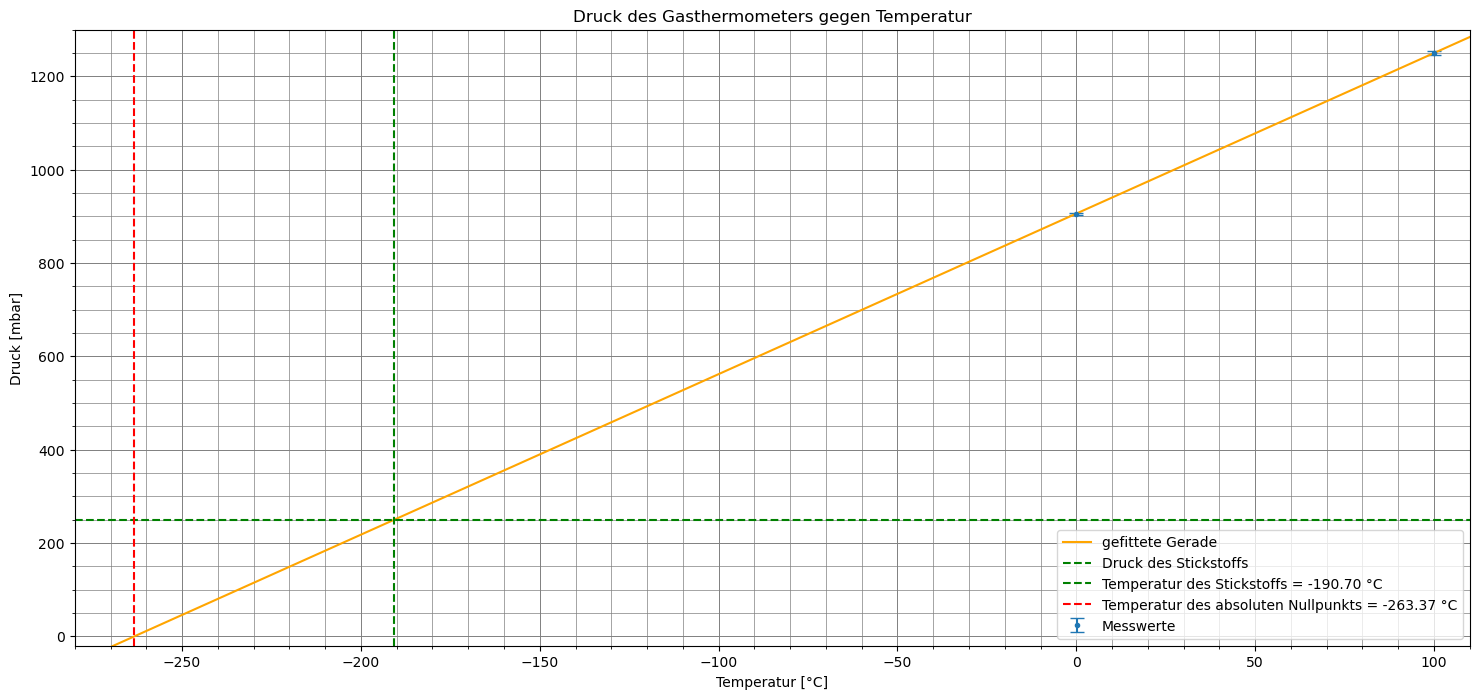
\includegraphics[width=\textwidth]{img/Eichkurve1.png}
    \caption{Druckwerte des Gasthermometers bei 0 °C und 100 °C.}
    \label{fig:plot1}
\end{figure}

Die Eichkurve beträgt die Geradengleichung: 
\begin{equation}
    p(T) = \qty{3.44}{\milli\bar\per\degreeCelsius} \cdot T + \qty{906}{\milli\bar}
\end{equation}

Die Punkte aus der Geradengleichung besitzen keine relevanten Fehler, da die Eichung nur mit zwei Punkten durchgeführt wurde.\footnote{Ja ich weiss eingentilch noch die beiden anderen Eichgeraden zeichnen aber das war mir zu blöd}
Die aus der Geradengleichung berechneten Temperaturen sind:

\begin{table}[H]
    \centering
    \caption{Berechnete Temperaturen aus der Eichgerade.}
    \begin{tabular}{ccc}
        \toprule
        \textbf{Messung} & \textbf{Druck $p$ [mbar]} & \textbf{Temperatur $T$ [°C]} \\
        \midrule
        0 Grad Wasser & 906 & 0.0 \\
        siedendes Wasser & 1250 & 100.0 \\
        Stickstoff & 250 & -190.70 \\
        Druck bei 0 bar & 0 & -263.37 \\
        \bottomrule
    \end{tabular}
\end{table}

Der Literaturwert von flüssigem Stickstoff beträgt $T_\text{Stickstoff} = -195.79\,\si{\degreeCelsius}$, was eine Abweichung von $\Delta T = 5.09\,\si{\degreeCelsius}$ ergibt. 

\subsection{Eichung mit dem Literaturwert von Flüssigem Stickstoff}

Nun wird dieser Literaturwert mit unserem Druckwert von $p_\text{Stickstoff} = 250\,\si{\milli\bar}$ geeicht. 

Die neue Gerade lautet:
\begin{equation}
    \num{3.376(23)} * T + \num{909.8(2.8)}
\end{equation}

Damit ergibt sich die Temperatur bei 0 K:
\begin{equation}
    T_0 = \frac{0 - \num{909.8(2.8)}}{\num{3.376(23)}} \approx \num{-269.5(2.0)} = \qty{3.7(2.0)}{\degreeCelsius}
\end{equation}

Die Temperatur des absoluten Nullpunkts beträgt also $T_0 = \qty{-269.5(2.0)}{\degreeCelsius}$, was eine Abweichung von $\Delta T = 3.7\,\si{\degreeCelsius}$ zum Literaturwert von $T_\text{0,lit} = -273.15\,\si{\degreeCelsius}$ ergibt. ($\Rightarrow 1.85\sigma$)

Der gemessene Druck bei Trockeneis beträgt $p_\text{Trockeneis} = \qty{651(2.1)}{\milli\bar}$, was bei der Eichkurve eine Temperatur von $T_\text{Trockeneis} = \qty{76.7(1.2)}{\degreeCelsius} = \qty{196.5(1.2)}{\kelvin}$ ergibt.

\begin{figure}[H]
    \centering
    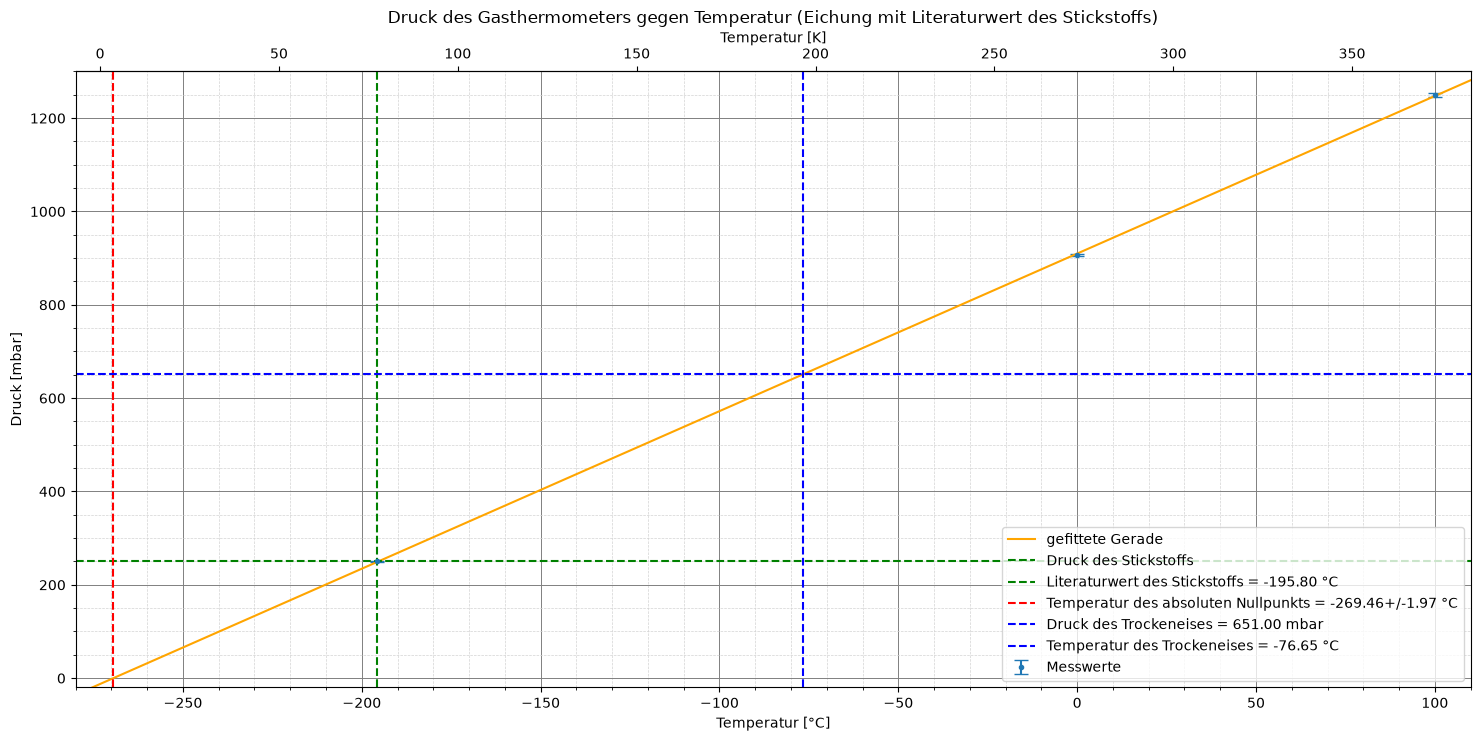
\includegraphics[width=\textwidth]{img/Eichkurve A2.png}
    \caption{Neue Eichkurve mit dem Literaturwert von flüssigem Stickstoff}
    \label{fig:EichkurveA2}
\end{figure}

\subsection{Temperaturbestimmung mit dem Gasthermometer und der Eichkurve}
Die abgelesenen Drücke aus dem Messprotokoll betragen:
\begin{table}[H]
    \centering
    \caption{Messwerte der Temperaturmessung bis 100\,°C im Wasserbad.}
    \begin{tabular}{cc}
        \toprule
        \textbf{Druck [mbar]} & Pyrometer\\
        \midrule
        \num{950.0(2.1)} & 9.3 \\
        \num{980.4(2.1)} & 19.8 \\
        \num{1017.0(2.1)} & 29.9 \\
        \num{1048.0(2.1)} & 40.2 \\
        \num{1081.0(2.1)} & 48.5 \\
        \num{1114.0(2.1)} & 58.6 \\
        \num{1146.0(2.1)} & 67.9 \\
        \num{1182.8(2.1)} & 78.0 \\
        \num{1211.0(2.1)} & 84.0 \\
        \num{1241.0(2.1)} & 90.0 \\
        \bottomrule\label{Messwerte}
    \end{tabular}
\end{table}

Die Temperaturen werden mit der Eichkurve \ref{fig:EichkurveA2} berechnet:
\begin{figure}[H]
    \centering
    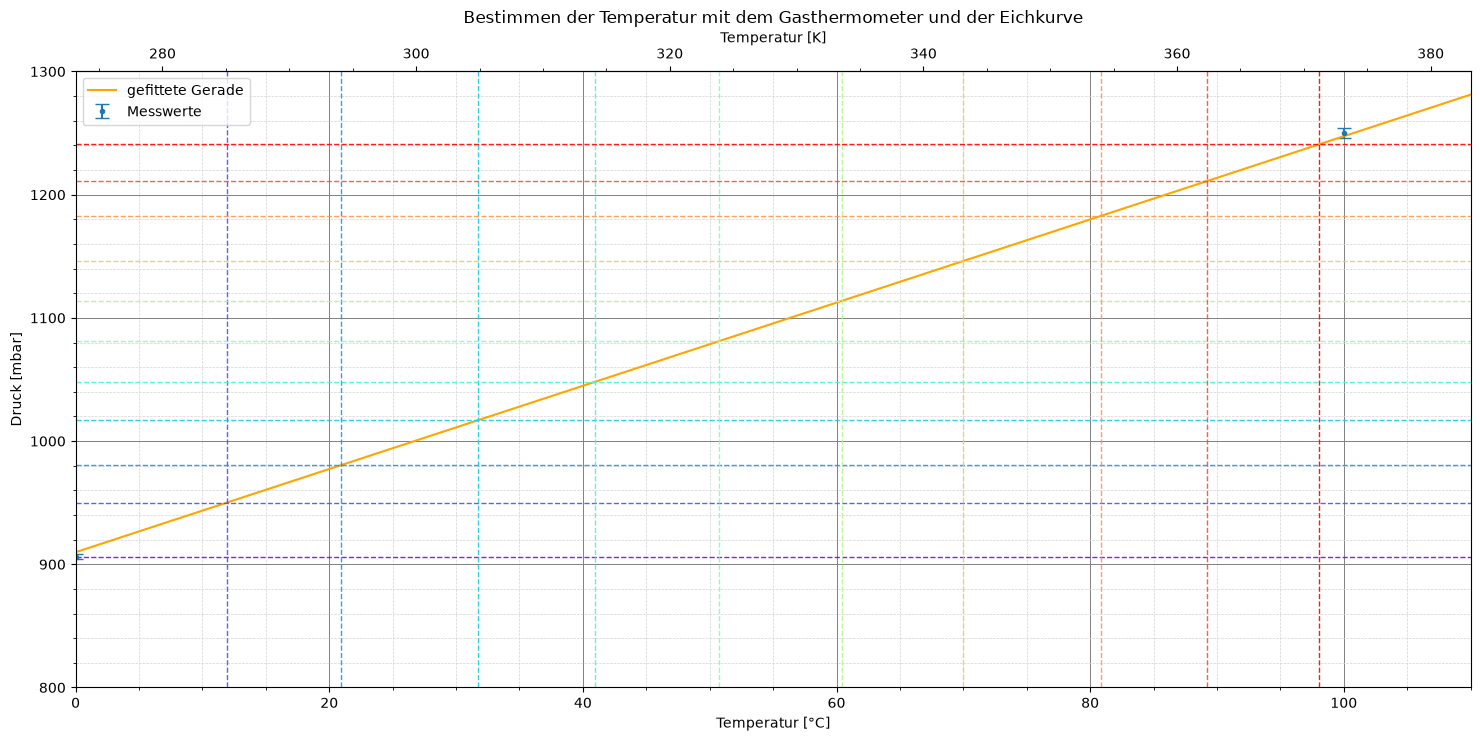
\includegraphics[width=\textwidth]{img/Eichkurve A3.png}
    \caption{Bestimmung der Temperatur}
    \label{fig:EichkurveA3}
\end{figure}

Die berechneten Temperaturen betragen:
\begin{table}[H]
    \centering
    \caption{Berechnete Temperaturen aus der Eichkurve.}
    \begin{tabular}{cc}
        \toprule
        \textbf{Druck [mbar]} & \textbf{Temperatur [°C]} \\
        \midrule
        \num{906(2.1)} & \num{0} \\
        \num{950.0(2.1)} & \num{11.9(1.1)} \\
        \num{980.4(2.1)} & \num{20.9(1.1)} \\
        \num{1017.0(2.1)} & \num{31.7(1.1)} \\
        \num{1048.0(2.1)} & \num{40.9(1.1)} \\
        \num{1081.0(2.1)} & \num{50.7(1.1)} \\
        \num{1114.0(2.1)} & \num{60.5(1.2)} \\
        \num{1146.0(2.1)} & \num{69.9(1.2)} \\
        \num{1182.8(2.1)} & \num{80.8(1.2)} \\
        \num{1211.0(2.1)} & \num{89.2(1.2)} \\
        \num{1241.0(2.1)} & \num{98.1(1.3)} \\
        \bottomrule
    \end{tabular}
\end{table}

\begin{resultbox}
    Die Eichung des Gasthermometers mit dem Literaturwert von flüssigem Stickstoff ergibt eine Abweichung von $\Delta T = 3.7\,\si{\degreeCelsius}$ zum Literaturwert des absoluten Nullpunkts.
\end{resultbox}


\subsection{Messung mit dem Widerstandthermometer PT100}
Der Fehler des Pt100-Aufbaus beträgt $\Delta U = 0.08\% + 0.2\,\text{mV}$, was bei einer Spannung von $U = 100\,\text{mV}$ einen Fehler von $\Delta U = 0.28\,\text{mV}$ ergibt.

Der Widerstand errechnet sich mit dem Ohmschen Gesetz:
\begin{equation}
    R = \frac{U}{I}
\end{equation}
Bei Uns beträgt der Strom $I = 1\,\text{mA}$, somit entspricht der Widerstand genau der Spannung in mV. Die Messwerte aus dem Messprotkoll betragen:

\begin{table}[H]
    \centering
    \caption{Messwerte der Temperaturmessung bis 100\,°C im Wasserbad.}
    \begin{tabular}{cc}
        \toprule
        \textbf{Spannung [mV]} & \textbf{Temperatur [°C] laut vorheriger Aufgabe}\\
        \midrule
        \num{99.8(0.28)} & \num{0}\\
        \num{104.50(0.29)} & \num{11.9(1.1)}\\
        \num{108.1(0.29)} & \num{20.9(1.1)}\\
        \num{111.7(0.29)} & \num{31.7(1.1)}\\  
        \num{115.5(0.3)} & \num{40.9(1.1)}\\
        \num{119.2(0.3)} & \num{50.7(1.1)}\\
        \num{123.0(0.3)} & \num{60.5(1.2)}\\
        \num{126.8(0.3)} & \num{69.9(1.2)}\\
        \num{130.8(0.3)} & \num{80.8(1.2)}\\ 
        \num{134.3(0.3)} & \num{89.2(1.2)}\\ 
        \num{137.9(0.4)} & \num{98.1(1.3)}\\ 
    \bottomrule
    \end{tabular}\label{Messwerte pt100}
\end{table}

Damit ergibt sich folgende Eichkurve für das Pt100-Thermometer:
\begin{figure}[H]
    \centering
    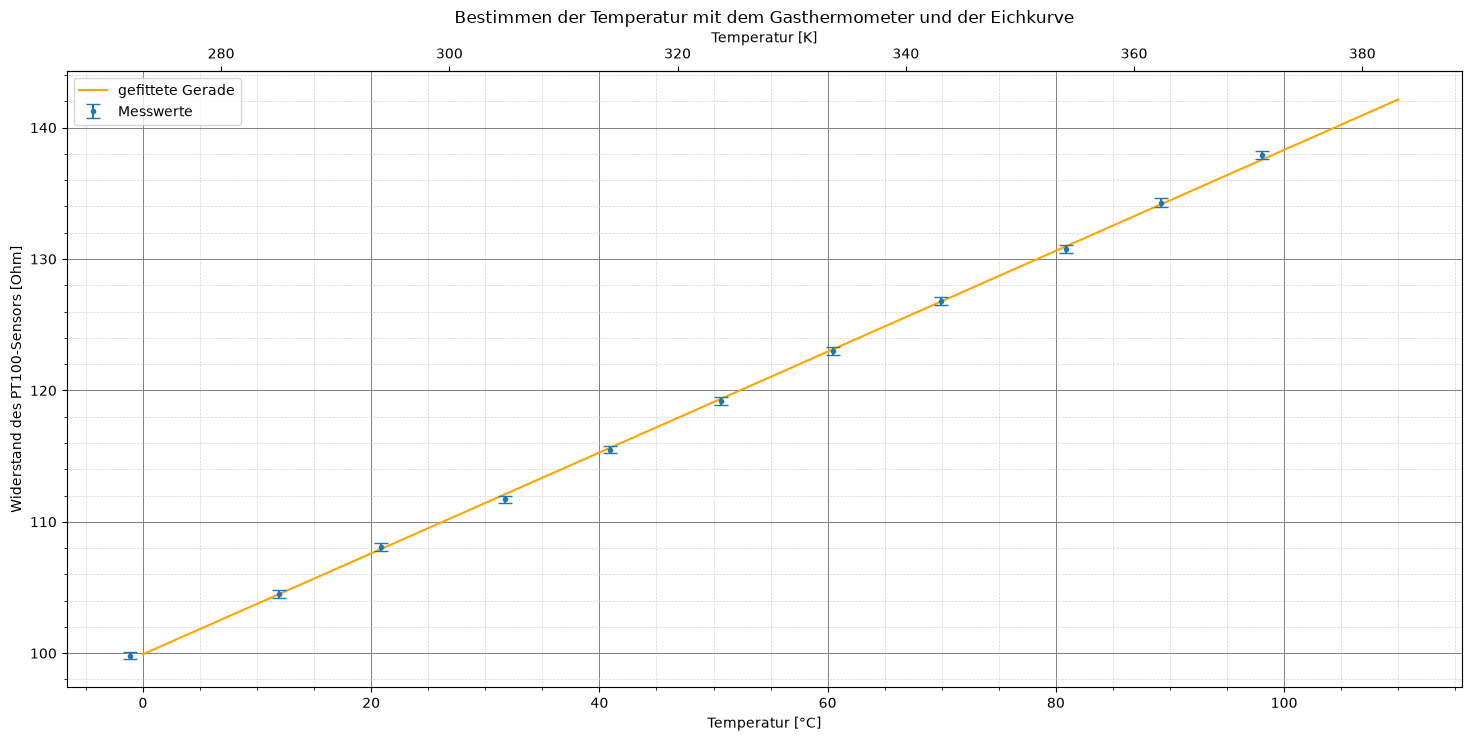
\includegraphics[width=\textwidth]{img/Eichkurve Pt100.png}
    \caption{Eichkurve für das Pt100-Thermometer.}
    \label{fig:EichkurvePt100}
\end{figure}

Die Geradengleichung lautet:
\begin{equation}
    R(T) = \num{0.3838(24)} * T + \num{99.92(14)} \label{eq:GeradengleichungPt100}
\end{equation}

Durch linearisierung der Gleichung für den Widerstand des Pt100-Thermometers \ref{eq:Widerstandpt100} ergibt sich die Gleichung:
\begin{equation}
    R(T) = R_0\cdot AT + R_0
\end{equation}

Mit Koeffizientenvergleich ergibt sich:
\begin{align}
    R_0 &= \num{99.92(14)}\\
    R_0\cdot A &= \num{0.3838(24)} \Rightarrow A \approx \num{3.838(24)e-3}
\end{align}

Die Literaturwerte betragen $A_\text{lit} = \num{3.9083e-3}$, $R_0 = 100\,\Omega$. Die Abweichung beträgt:
\begin{align}
    \Delta A &= \num{3.9083e-3} - \num{3.838(24)e-3} = \num{7.03e-5} \approx 2.9\sigma\\
    \Delta R_0 &= 100 - \num{99.92(14)} = \num{0.08} \approx 0.57\sigma
\end{align}


\begin{resultbox}[Ergebnis]
    Die Eichung des Pt100-Thermometers ergibt eine Abweichung von $\Delta A \approx 2.9\sigma$ und $\Delta R_0 \approx 0.57\sigma$ im Vergleich zu den Literaturwerten.
\end{resultbox}


\subsection{Temperaturmessung mit dem Pyrometer}

Nun werden die Messwerte des Pyrometers aus dem Messprotokoll mit den berechneten Temperaturen aus der Eichkurve des Gasthermometers verglichen. 
Der Fehler des Pyrometers beträgt $\Delta T = 1\% + 2\,\si{\degreeCelsius}$.
Die Messwerte des Pyrometers betragen:
\begin{table}[H]
    \centering
    \caption{Messwerte des Pyrometers im Vergleich zu den berechneten Temperaturen aus der Eichkurve des Gasthermometers.}
    \begin{tabular}{cc}
        \toprule
        \textbf{Temperatur [°C] aus Gasthermometer} & \textbf{Temperatur [°C] aus Pyrometer} \\
        \midrule
        \num{0} & \num{-1(2.0)}\\
        \num{11.9(1.1)} & \num{9.3(2.2)}\\
        \num{20.9(1.1)} & \num{19.8(2.3)}\\
        \num{31.7(1.1)} & \num{29.9(2.5)}\\
        \num{40.9(1.1)} & \num{40.2(2.6)}\\
        \num{50.7(1.1)} & \num{48.5(2.8)}\\
        \num{60.5(1.2)} & \num{58.6(2.9)}\\
        \num{69.9(1.2)} & \num{67.9(3.0)}\\
        \num{80.8(1.2)} & \num{78(4)}\\
        \num{89.2(1.2)} & \num{84(4)}\\
        \num{98.1(1.3)} & \num{90(4)}\\
        \bottomrule
    \end{tabular}
\end{table}

Die Werte werden in einem Diagramm dargestellt:
\begin{figure}[H]
    \centering
    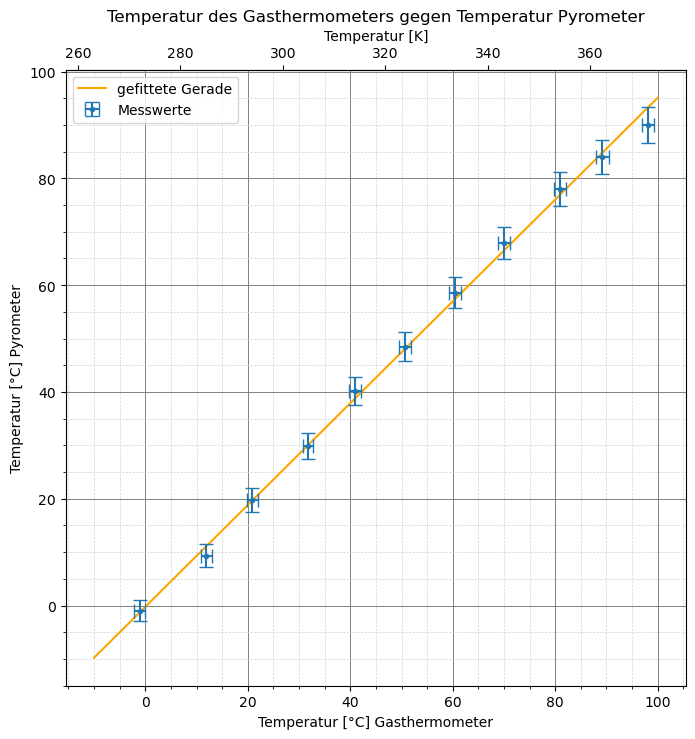
\includegraphics[width=\textwidth]{img/Pyrometervergleich.png}
    \caption{Vergleich der Messwerte des Pyrometers mit den berechneten Temperaturen aus der Eichkurve des Gasthermometers.}
    \label{fig:Pyrometervergleich}
\end{figure}

Die optimale Gerade durch die Messwerte des Pyrometers ergibt sich zu:
\begin{equation}
    T_\text{Pyrometer} = \num{0.953(25)} * T_\text{Gasthermometer} - \num{0.2(1.3)} \
\end{equation}

\begin{resultbox}[Ergebnis]
    Die Eichung des Pyrometers ergibt eine Abweichung von $\Delta m = 0.025$ in der Steigung und $\Delta b = 1.3$ in der y-Achsenabschnitt. Die Abweichung der Steigung von 1 beträgt $\Delta m = 0.047$, was einer Abweichung von $1.88\sigma$ entspricht.
\end{resultbox}



\section{Diskussion}

Im Rahmen dieses Versuchs konnten verschiedene Methoden der Temperaturmessung (Gasthermometer, Platin-Widerstandsthermometer, Pyrometer und Thermoelement) erfolgreich angewendet und auf ihre Genauigkeit sowie spezifische Fehlerquellen untersucht werden.

\paragraph{Gasthermometer und absoluter Nullpunkt}
Die Bestimmung des absoluten Nullpunkts durch Extrapolation der isochoren Druckänderung lieferte einen Wert von $T_0 = \qty{-269.5(2.0)}{\degreeCelsius}$. Mit einer Abweichung von $\Delta T = \qty{3.7}{\degreeCelsius}$ zum Literaturwert (\qty{-273.15}{\degreeCelsius}) liegt das Ergebnis in einem sehr guten Bereich, was sich auch in der geringen Signifikanz der Abweichung ($1.85\sigma$) widerspiegelt. Die leichte Überschätzung der Temperatur lässt sich durch systematische Fehlerquellen des Aufbaus erklären: Das "`schädliche Volumen"' in der Kapillare und im Drucksensor befand sich stets auf Raumtemperatur und nahm nicht an der thermischen Kontraktion bzw. Expansion im Wasserbad teil. Zudem wurde die thermische Volumenänderung des Glaskolbens selbst vernachlässigt. 

Auch die Messung der Sublimationstemperatur von Trockeneis lieferte mit \qty{-76.7(1.2)}{\degreeCelsius} ein sehr gutes Ergebnis, das nah am Literaturwert von ca. \qty{-78.5}{\degreeCelsius} liegt. Ein weiterer systematischer Fehler entstammt der Skript-Vorgabe, den Siedepunkt über einen einfachen Dreisatz des Luftdrucks auf Normalbedingungen zu korrigieren, anstatt die physikalisch korrekte Dampfdruckkurve (Clausius-Clapeyron-Gleichung) zu verwenden. 

\paragraph{Platin-Widerstandsthermometer (Pt100)}
Die Kalibrierung des Pt100-Thermometers lieferte für den Nennwiderstand bei \qty{0}{\degreeCelsius} einen exzellenten Wert von $R_0 = \qty{99.92(14)}{\Omega}$. Die Abweichung zum Idealwert von $100\,\si{\Omega}$ ist mit $0.57\sigma$ statistisch nicht signifikant. Die Vierleiterschaltung hat hier erwartungsgemäß die Zuleitungswiderstände erfolgreich eliminiert. 

Der lineare Temperaturkoeffizient $A$ weicht mit $A = \qty{3.838e-3}{\degreeCelsius}^{-1}$ jedoch um $2.9\sigma$ vom Literaturwert ab. Diese signifikante Abweichung ist primär auf die in der Auswertung vorgenommene Linearisierung zurückzuführen. In der Realität besitzt die $R(T)$-Kurve von Platin einen quadratischen Term ($B \cdot T^2$), der bei \qty{100}{\degreeCelsius} zwar klein ist, das lineare Modell jedoch systematisch verfälscht. Zudem baut diese Messung auf den Temperaturwerten der vorherigen Gasthermometer-Eichung auf, wodurch sich dessen systematische Fehler (z.\,B. das schädliche Volumen) in diese Messreihe fortpflanzen.

\paragraph{Pyrometer}
Das Pyrometer zeigte bei Raumtemperatur und \qty{0}{\degreeCelsius} noch eine gute Übereinstimmung mit dem Gasthermometer, unterschätzte die Temperatur jedoch bei höheren Werten zunehmend. Dies zeigt sich deutlich in der linearen Regression, deren Steigung $m = \num{0.953(25)}$ um $1.88\sigma$ vom idealen Wert $m=1$ abweicht. Bei kochendem Wasser zeigte das Pyrometer lediglich \qty{90(4)}{\degreeCelsius} an. 

Dieser systematische Fehler ist ein klassisches Problem der berührungslosen Infrarotmessung über erhitzten Flüssigkeiten: Der aufsteigende Wasserdampf absorbiert einen Teil der emittierten Infrarotstrahlung, bevor diese den Sensor erreicht. Die im Skript empfohlene schräge Messung konnte diesen Effekt offenbar nicht vollständig kompensieren. Zudem hängt die Genauigkeit des Pyrometers stark vom korrekten Emissionsgrad $\epsilon$ der Oberfläche ab, welcher durch Reflexionen der Umgebung (z.\,B. Beleuchtung im Praktikumsraum) verfälscht werden kann.



\clearpage

\listoffigures


\listoftables

\begin{thebibliography}{5}
    \bibitem{PAPskript} Dr. J.Wagner, \emph{Physikalisches Anfängerpraktikum}, Stand 11/2024
    \bibitem{ilberg1988physikalisches} W. Ilberg, M. Krötzsch, \emph{Physikalisches Praktikum für Anfänger}, BSB B. G. Teubner Verlagsgesellschaft, Leipzig (1985).
\end{thebibliography}


\appendix
\section{Anhang: Eichtabellen}
\begin{figure}[H]
    \centering
    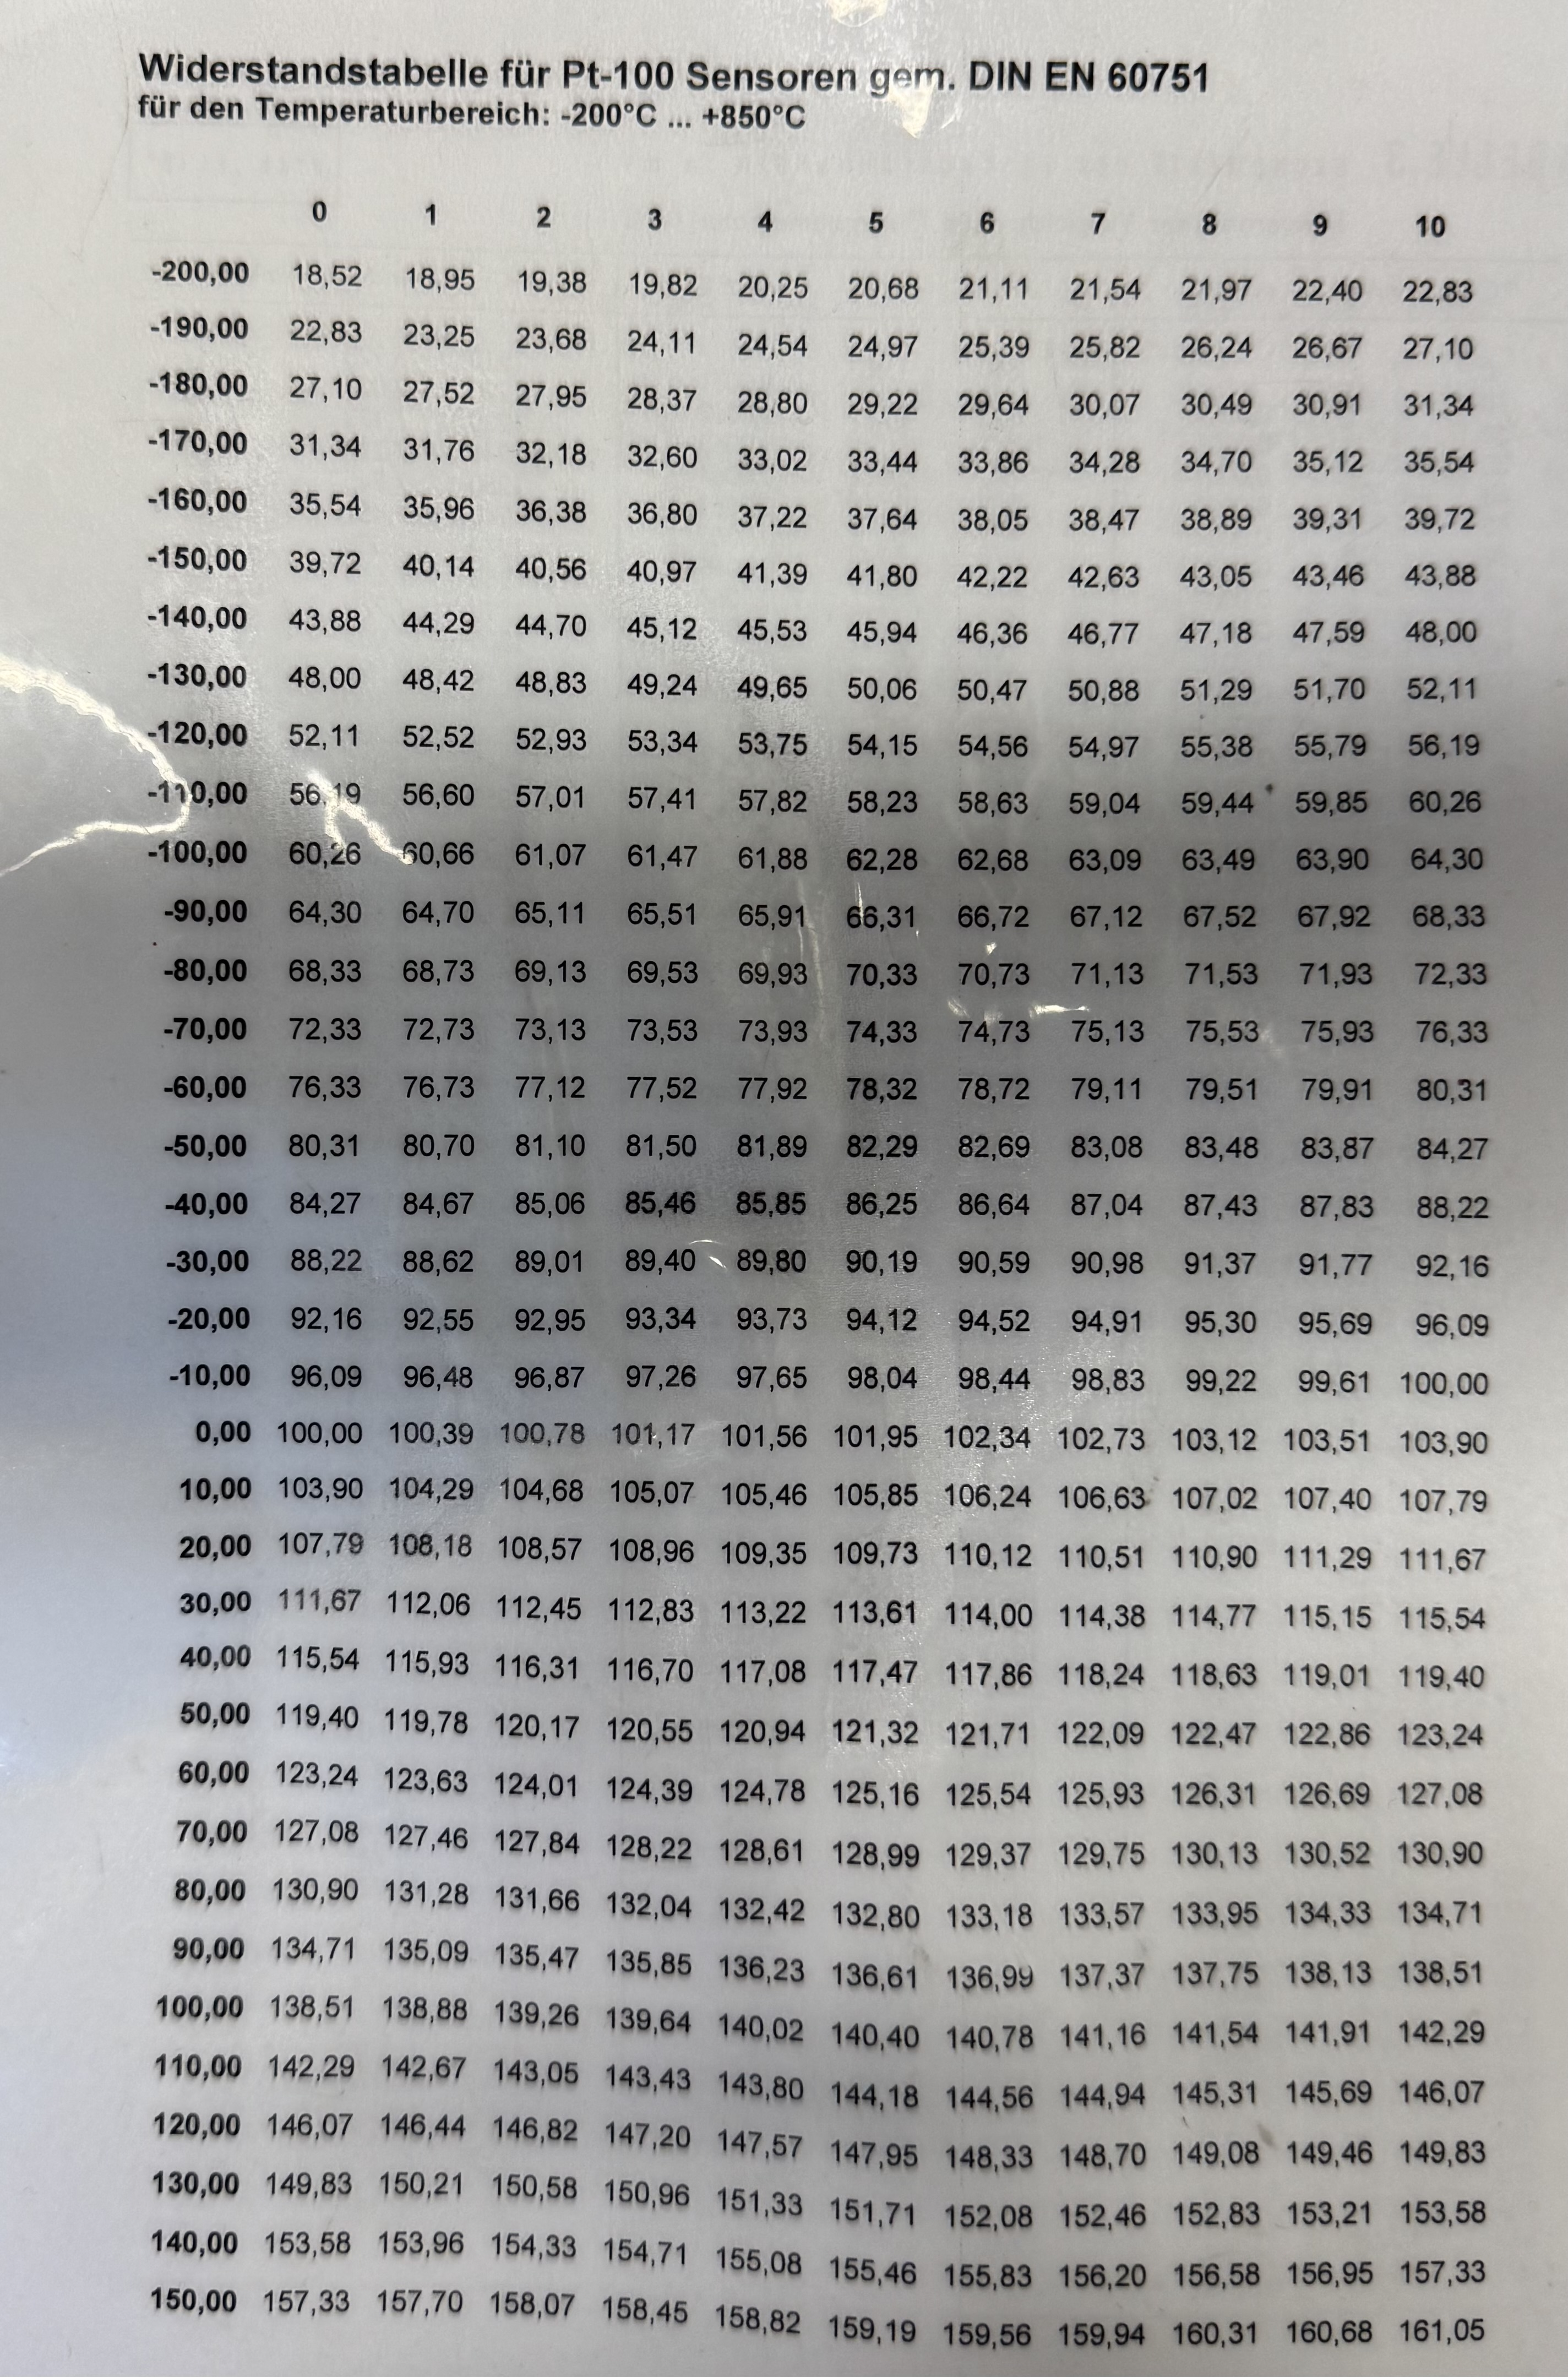
\includegraphics[width=0.8\textwidth]{img/Eichtabelle1.jpeg}
    \caption{Eichtabelle für das Pt100-Element.}
    \label{fig:Eichtabelle1}
\end{figure}

\begin{figure}[H]
    \centering
    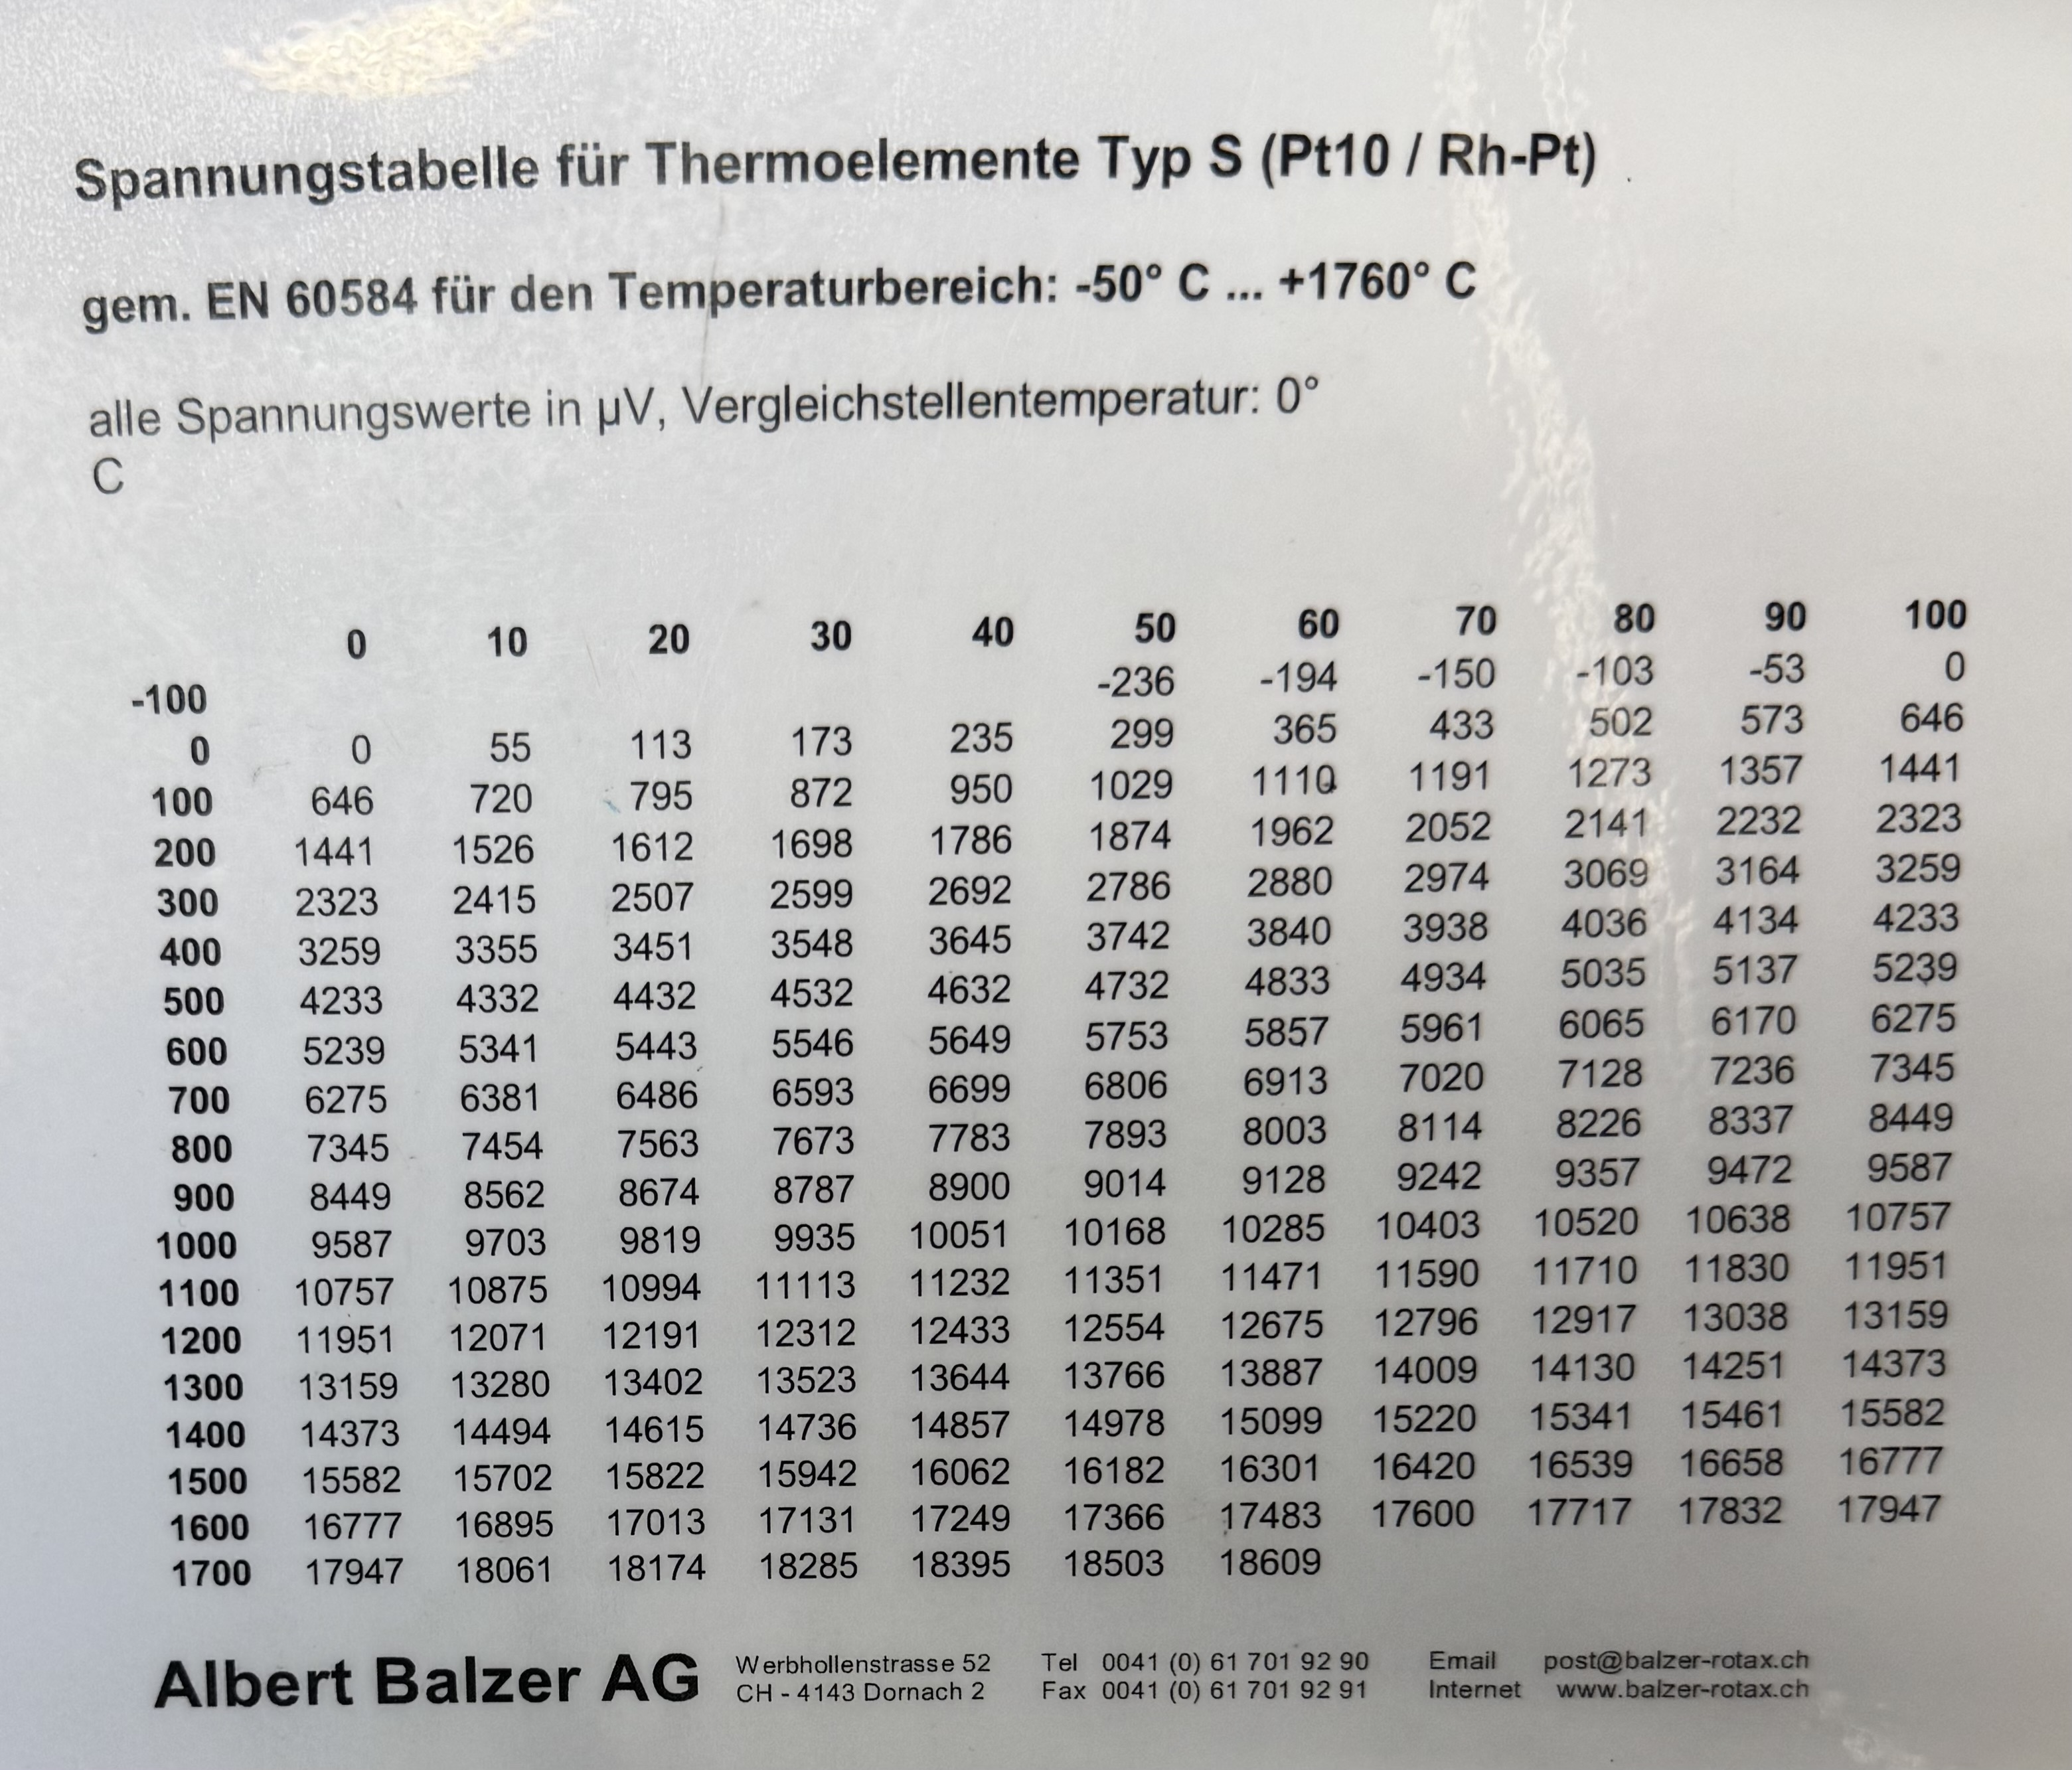
\includegraphics[width=0.8\textwidth]{img/Eichtabelle2.jpeg}
    \caption{Eichtabelle für das PtRh - Typ B.}
    \label{fig:Eichtabelle2}
\end{figure}

\begin{figure}[H]
    \centering
    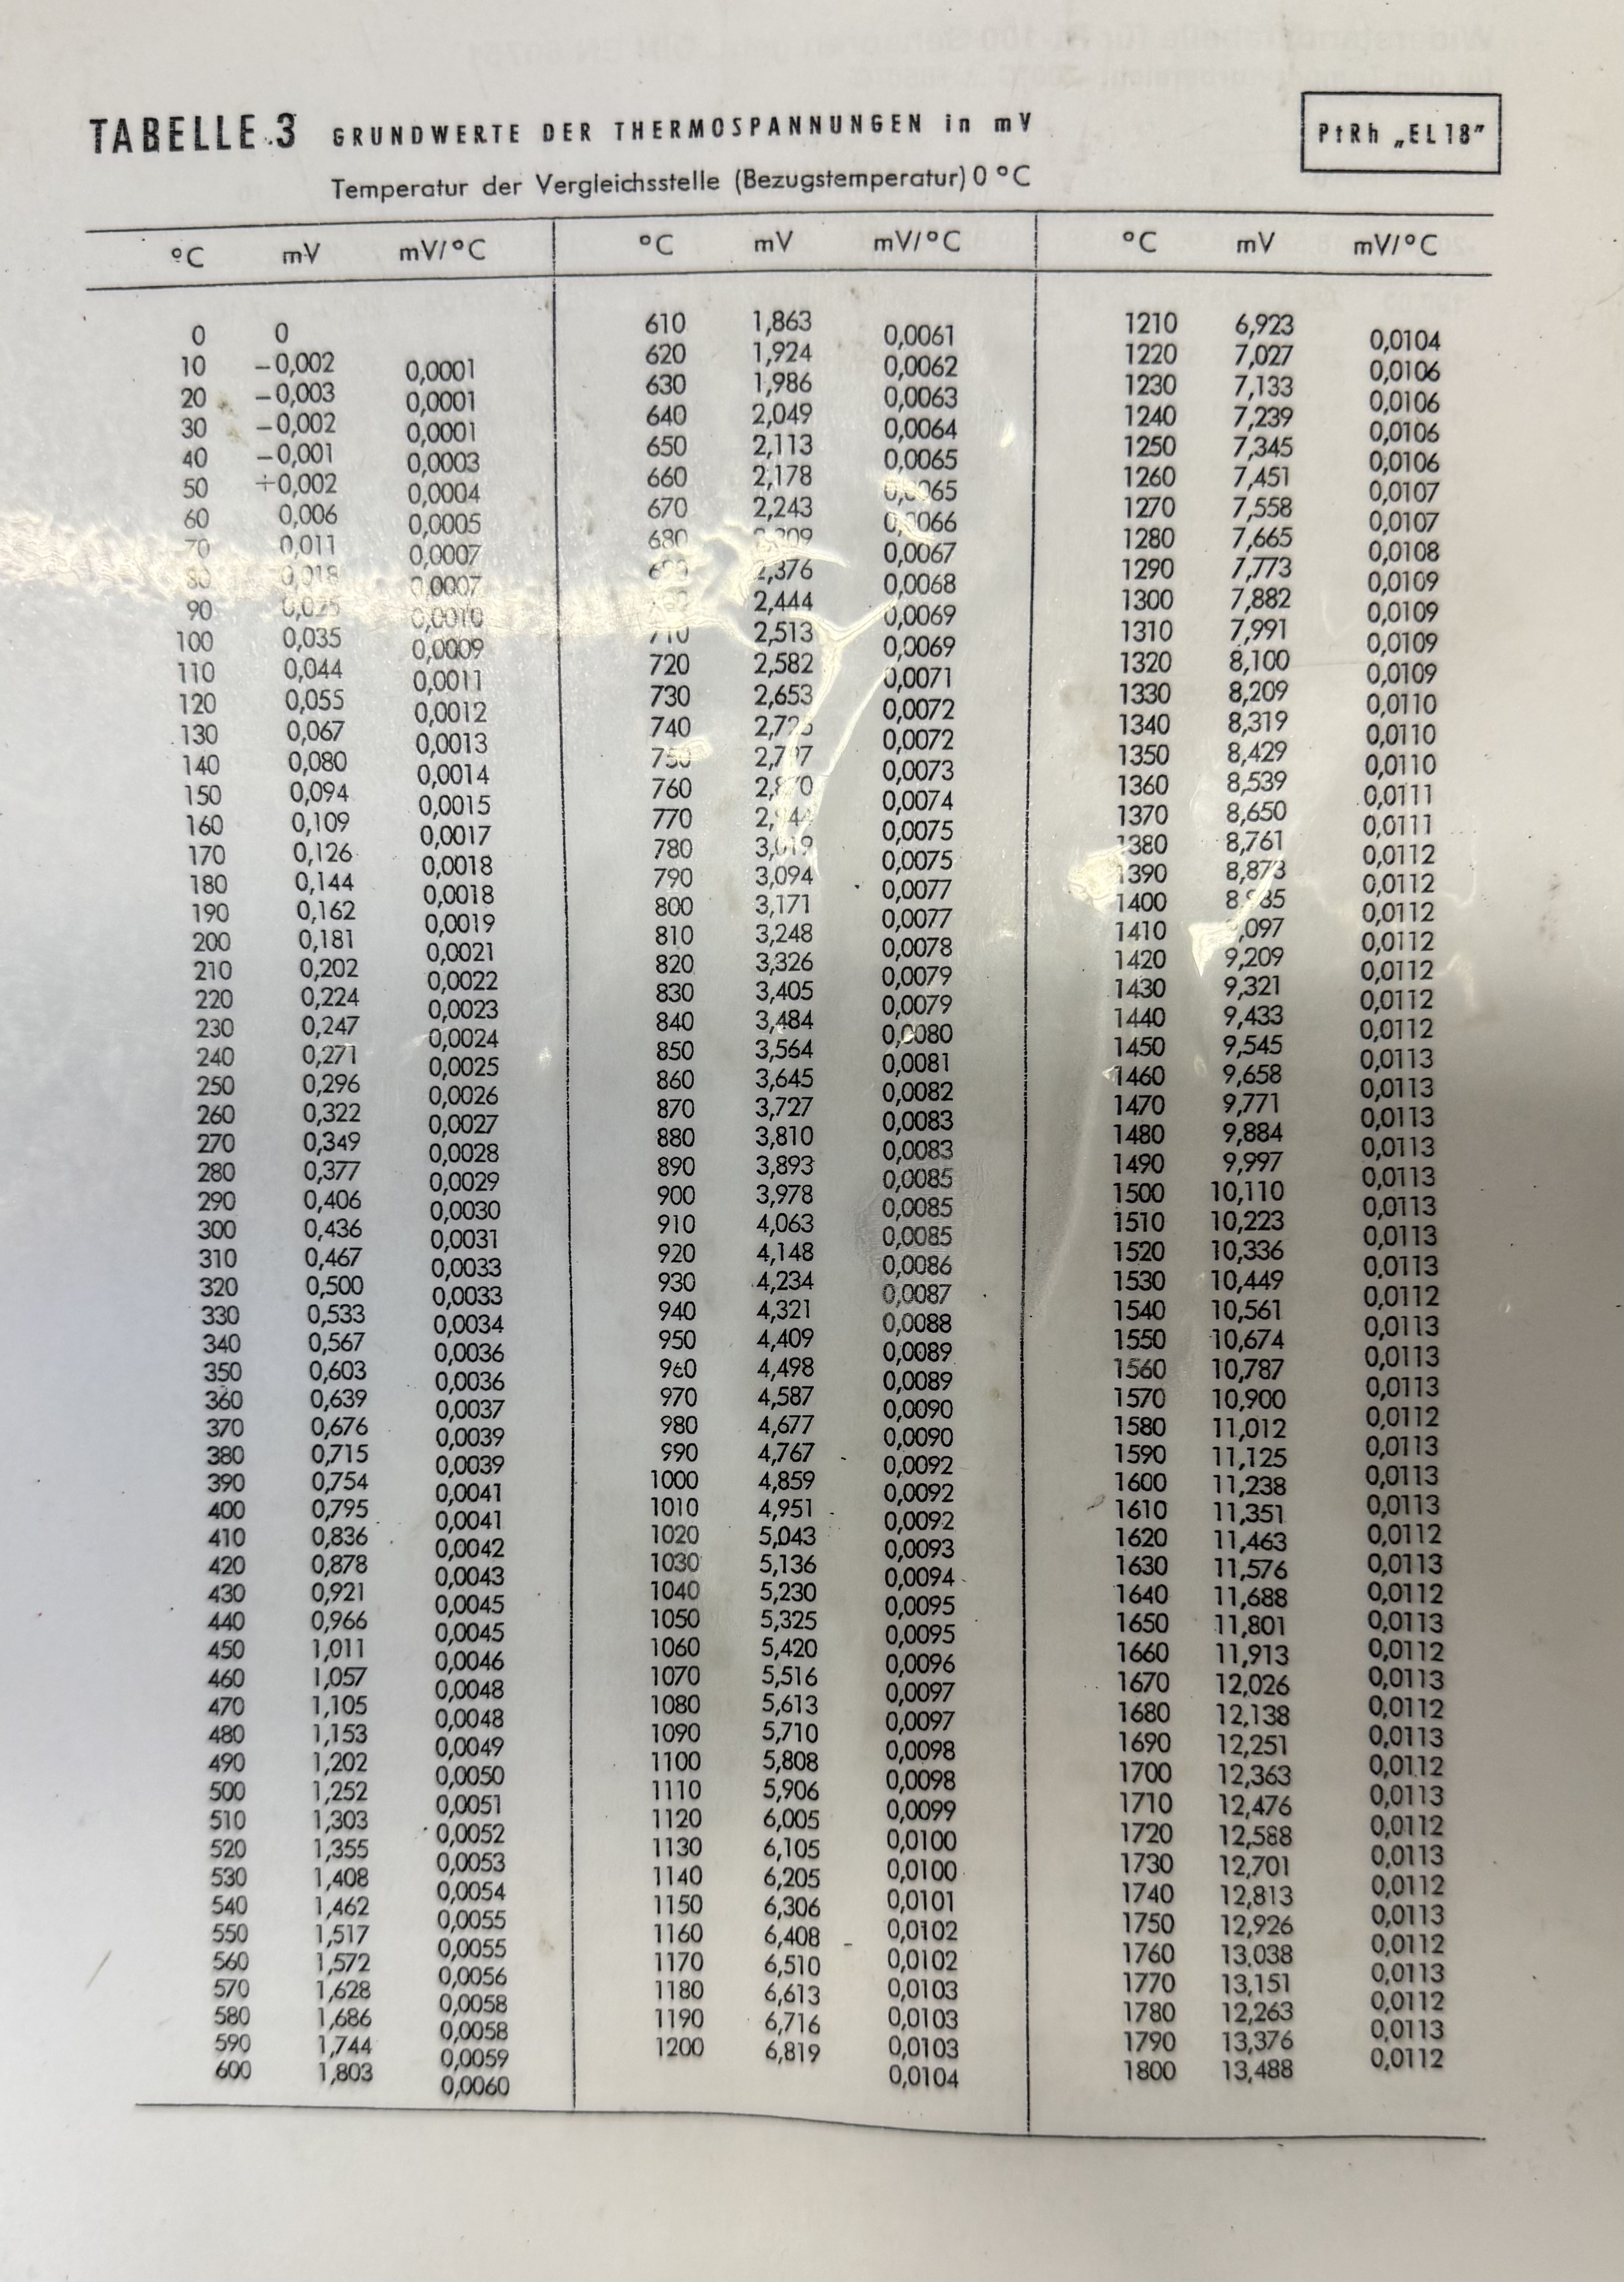
\includegraphics[width=0.8\textwidth]{img/Eichtabelle3.jpeg}
    \caption{Eichtabelle für das PtRh - Typ S.}
    \label{fig:Eichtabelle3}
\end{figure}

\section{Anhang: Code}
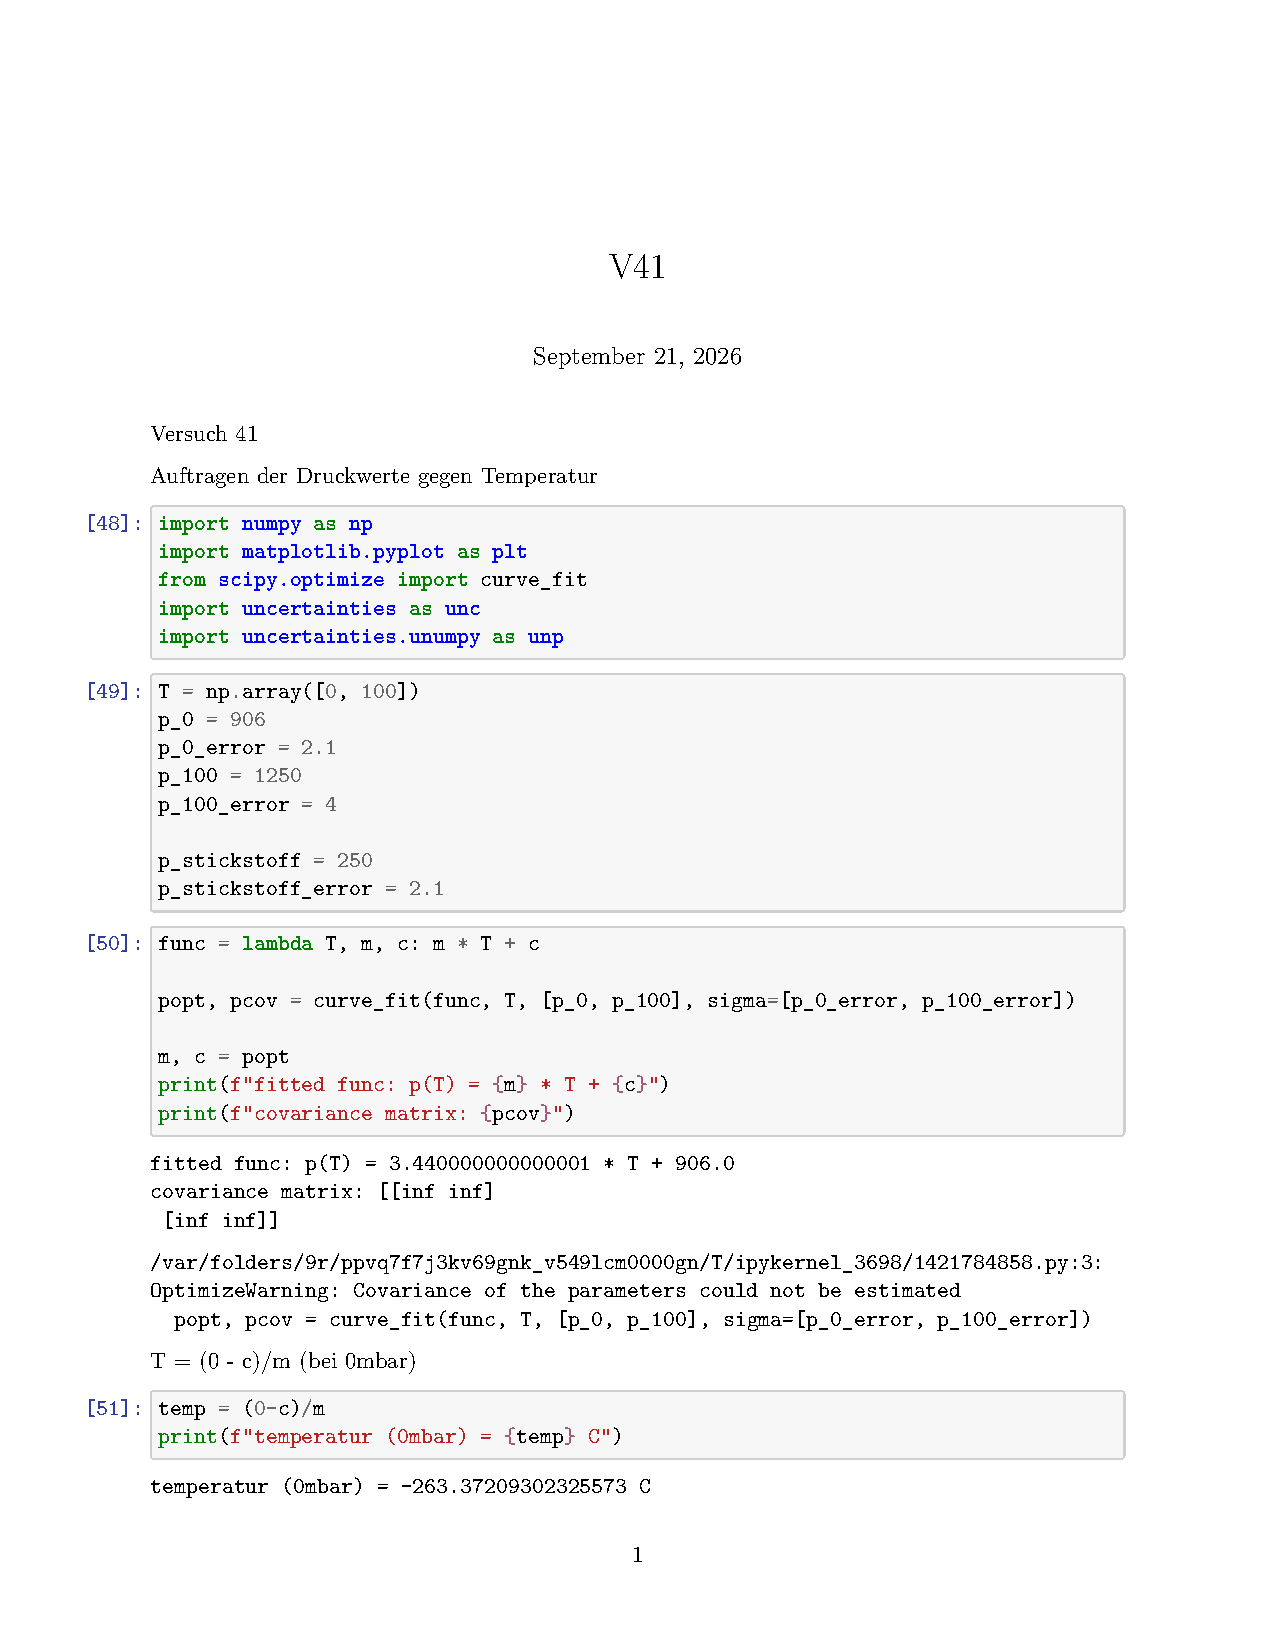
\includepdf[
    pages=-,
    width=\textwidth,
    height=0.95\textheight,
    keepaspectratio,
    pagecommand={\thispagestyle{scrheadings}},
]
    {code/V41.pdf}


\begin{comment}

\begin{table}[H]
    \centering
    \caption{Mess- und Geräteparameter für die exemplarische Berechnung (Messung 28).}
    \label{tab:parameter_messung_28}
    \begin{tabular}{ll}
        \toprule
        \textbf{Größe} & \textbf{Wert} \\
        \midrule
        Fallstrecke & $s_1 = 10\,\text{Skt} = 5.00  10^{-4}\,\text{m}$ \\
        Fallzeit & $t_1 = 11.85\,\text{s}$ \\
        Steigstrecke & $s_2 = 10\,\text{Skt} = 5.00  10^{-4}\,\text{m}$ \\
        Steigzeit & $t_2 = 18.19\,\text{s}$ \\
        Skalenteilung & $1\,\text{Skt} = 5.00  10^{-5}\,\text{m}$ \\
        Kondensatorspannung & $U = 500\,\text{V}$ \\
        Plattenabstand & $d = 6.00  10^{-3}\,\text{m}$ \\
        Luftdruck & $p = 100285\,\text{Pa}$ \\
        Erdbeschleunigung & $g = 9.81\,\frac{\text{m}}{\text{s}^2}$ \\
        Dichtedifferenz & $\rho = \rho_{\text{Öl}} - \rho_{\text{Luft}} = 871.21\,\frac{\text{kg}}{\text{m}^3}$ \\
        Unkorrigierte Luftviskosität & $\eta_0 = 1.81  10^{-5}\,\text{Pa}\text{s}$ \\
        Cunningham-Konstante & $b = 7.78  10^{-3}\,\text{Pa}\text{m}$ \\
        \bottomrule
    \end{tabular}
\end{table}
\end{comment}


\end{document}